\section[SOM]{Self Organized Maps}
El código se basó en la documentación cargada de la página de Scikit-learn de Python.

\subsection[Proceso]{Proceso}
Para el método manual se siguieron los siguientes pasos:
\begin{itemize}
    \item[1.] Carga de los datos de Iris de \texttt{sklearn.datasets}, de la cual se toman únicamente los datos de longitud y ancho del sépalo.
    \item[2.] Se crea una instancia de un SOM con una matriz 3x1 y una dimensión de 2, que corresponde a las características seleccionadas de los datos de Iris.
    \item[3.] Después del entrenamiento, se generan predicciones con el SOM para los datos de entrada utilizando \texttt{predict()}. Gracias al entrenamiento previo, el SOM los clasifica automáticamente.
\end{itemize}

\subsection[Resultados]{Resultados obtenidos}

El diagrama obtenido previo al entrenamiento de SOM:

\begin{center}
    \begin{figure}[!ht]
        \centering
        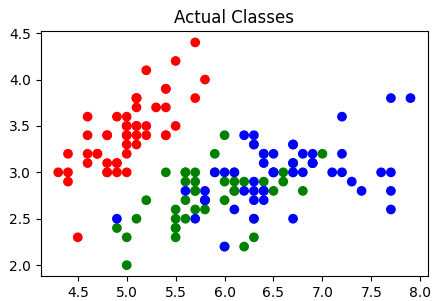
\includegraphics[scale=0.67]{Previo_SOM.png}
        \caption{Datos previos al entrenamiento de SOM}
    \end{figure}
\end{center}

Datos después del entrenamiento del modelo y utilizando el modelo predictivo:

\begin{center}
    \begin{figure}[!ht]
        \centering
        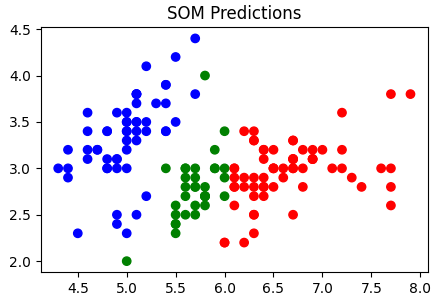
\includegraphics[scale=0.67]{After_SOM.png}
        \caption{Datos después del entrenamiento de SOM}
    \end{figure}
\end{center}
